\documentclass[tikz,border=5pt]{standalone}
\usepackage{fontspec}
\setmainfont{Times New Roman}
\usepackage{unicode-math}
\setmathfont{Cambria Math}
\usetikzlibrary{shapes.geometric,shapes.misc,positioning,fit,backgrounds,arrows.meta,calc}

\begin{document}
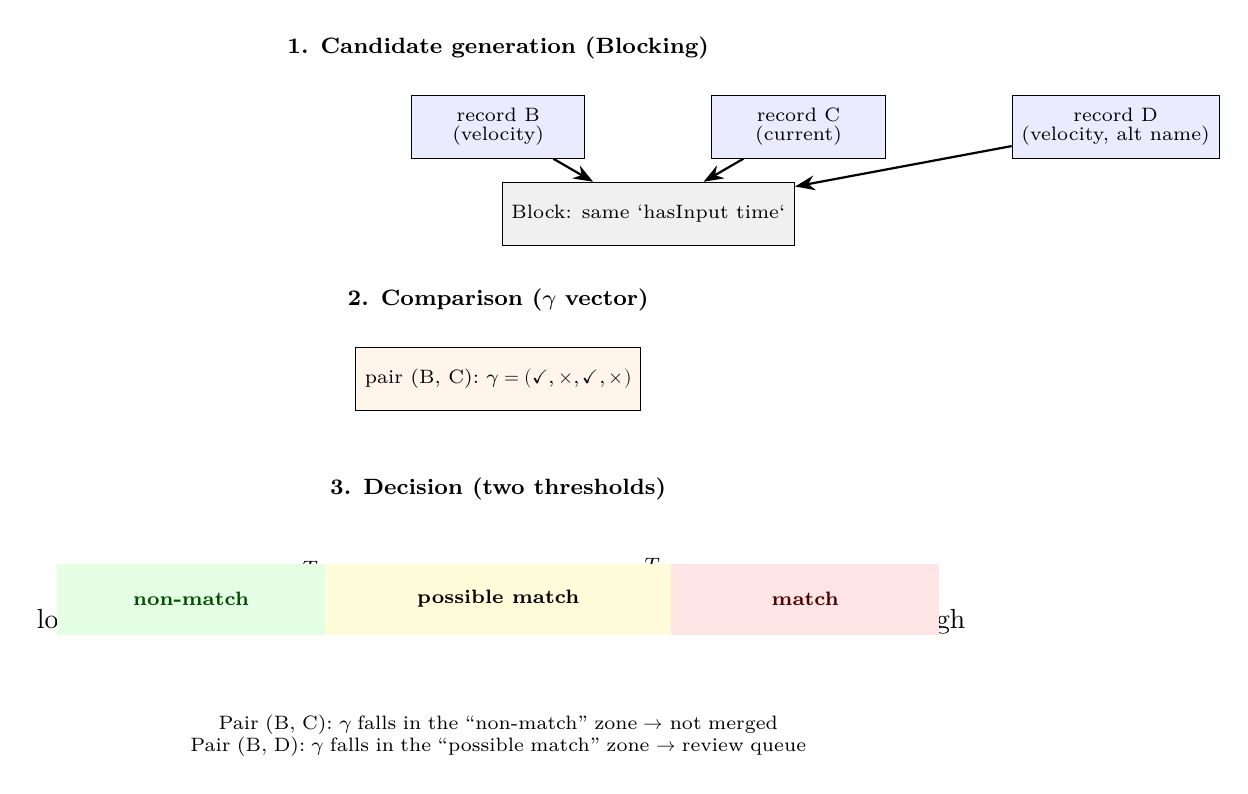
\begin{tikzpicture}[
    node distance=1.2cm and 1.6cm,
    rec/.style={rectangle, draw, minimum width=2.2cm, minimum height=0.8cm, align=center, font=\scriptsize},
    label/.style={font=\scriptsize\itshape, text=gray!60!black},
    arrow/.style={-{Stealth[length=2.5mm]}, thick},
    zone/.style={font=\scriptsize\bfseries},
    phase/.style={font=\footnotesize\bfseries},
]

% ====== Candidate generation / blocking ======
\node[phase, font=\footnotesize\bfseries] (genTitle) at (0, 3.6) {1. Candidate generation (Blocking)};
\node[rec, fill=blue!8] (r1) at (0, 2.6) {record B\\[-1pt]\scriptsize(velocity)};
\node[rec, fill=blue!8, right=of r1] (r2) {record C\\[-1pt]\scriptsize(current)};
\node[rec, fill=blue!8, right=of r2] (r3) {record D\\[-1pt]\scriptsize(velocity, alt name)};

\node[rec, fill=gray!12, below=0.7cm of $(r1)!0.5!(r2)$] (blk) {Block: same `hasInput time`};
\draw[arrow] (r1) -- (blk);
\draw[arrow] (r2) -- (blk);
\draw[arrow] (r3) -- (blk);

% ====== Comparison ======
\node[phase, font=\footnotesize\bfseries] (cmpTitle) at (0, 0.4) {2. Comparison ($\gamma$ vector)};
\node[rec, fill=orange!8, minimum width=3.6cm] (cmp) at (0, -0.6) {pair (B, C): $\gamma = (\checkmark, \times, \checkmark, \times)$};

% ====== Two thresholds ======
\node[phase, font=\footnotesize\bfseries] (decTitle) at (0, -2.0) {3. Decision (two thresholds)};

% draw a horizontal axis with three zones
\begin{scope}[yshift=-3.4cm]
  \draw[thick, -{Stealth[length=2.5mm]}] (-5.6, 0) -- (5.6, 0);
  \node[below] at (-5.6, 0) {low};
  \node[below] at (5.6, 0) {high};
  % low threshold
  \draw[thick] (-2.2, -0.12) -- (-2.2, 0.12) node[above, font=\scriptsize] {$T_{low}$};
  \draw[thick] (2.2, -0.12) -- (2.2, 0.12) node[above, font=\scriptsize] {$T_{high}$};
  % zones
  \fill[green!10] (-5.6, -0.45) rectangle (-2.2, 0.45);
  \fill[yellow!15] (-2.2, -0.45) rectangle (2.2, 0.45);
  \fill[red!10] (2.2, -0.45) rectangle (5.6, 0.45);
  \node[zone, text=black!70!green] at (-3.9, 0) {non-match};
  \node[zone] at (0, 0) {possible match};
  \node[zone, text=black!70!red] at (3.9, 0) {match};
\end{scope}

\node[font=\scriptsize, align=center, text width=9cm, below=0.15cm] (note) at (0, -4.6)
{Pair (B, C): $\gamma$ falls in the ``non-match'' zone $\rightarrow$ not merged\\
Pair (B, D): $\gamma$ falls in the ``possible match'' zone $\rightarrow$ review queue};

\end{tikzpicture}
\end{document}
